\documentclass[nojss]{jss}

\usepackage{setspace}
% \usepackage[sc]{mathpazo}
\usepackage{amsmath}
% \setcounter{secnumdepth}{2}
% \setcounter{tocdepth}{2}
%\usepackage{colortbl}

\usepackage{xcolor}
\usepackage{booktabs}

% For kable tables, these help.
\usepackage{floatrow}
\floatsetup[table]{capposition=bottom}
\floatplacement{table}{htb}
%%%%%%%%%%%%%%%%%%%%%%%%%%%%%%
%% declarations for jss.cls %%
%%%%%%%%%%%%%%%%%%%%%%%%%%%%%%
%\VignetteEngine{knitr::knitr}
%\VignetteIndexEntry{randomForestSRC-Survival}
%\VignetteIndexEntry{ggRandomForests: Survival with random forest}
%\VignetteKeywords{random forest, survival, VIMP, minimal depth}
%\VignetteDepends{ggRandomForests}
%\VignettePackage{ggRandomForests}

%% almost as usual
\author{John Ehrlinger \and Jeevanantham Rajeswaran \and Eugene H. Blackstone\\Cleveland Clinic }

\title{\pkg{ggRandomForests}: Exploring Random Forest Survival}

%% for pretty printing and a nice hypersummary also set:
\Plainauthor{Ehrlinger, Rajeswaran and Blackstone} %% comma-separated
\Plaintitle{ggRandomForests: Exploring Random Forest Survival} %% without formatting
\Shorttitle{Exploring Random Forest Survival}

%% an abstract and keywords
\Abstract{
Random forest~\citep{Breiman:2001} (RF) is a non-parametric statistical method requiring no distributional assumptions on covariate relation to the response. RF is a robust, nonlinear technique that optimizes predictive accuracy by fitting an ensemble of trees to stabilize model estimates. Random survival forests (RSF)~\citep{Ishwaran:2007a, Ishwaran:2008} are an extension of Breiman's RF techniques allowing efficient non-parametric analysis of time to event data. The \pkg{randomForestSRC} package~\citep{Ishwaran:RFSRC:2014} is a unified treatment of Breiman's random forest for survival, regression and classification problems.

Predictive accuracy makes RF an attractive alternative to parametric models, though complexity and interpretability of the forest hinder wider application of the method. We introduce the \pkg{ggRandomForests} package, tools for visually understand random forest models grown in \proglang{R}~\citep{rcore} with the \pkg{randomForestSRC} package. The \pkg{ggRandomForests} package is structured to extract intermediate data objects from \pkg{randomForestSRC} objects and generate figures using the \pkg{ggplot2}~\citep{Wickham:2009} graphics package.

This document is structured as a tutorial for building random forest for survival with the \pkg{randomForestSRC} package and using the \pkg{ggRandomForests} package for investigating how the forest is constructed. We analyse the Primary Biliary Cirrhosis of the liver data from a clinical trial at the Mayo Clinic~\citep{fleming:1991}. We demonstrate random forest variable selection using Variable Importance (VIMP)~\citep{Breiman:2001} and Minimal Depth~\citep{Ishwaran:2010}, a property derived from the construction of each tree within the forest. We will also demonstrate the use of variable dependence and partial dependence plots~\citep{Friedman:2000} to aid in the interpretation of RSF results. We then examine variable interactions between covariates using conditional variable dependence plots. Our aim is to demonstrate the strength of using Random Forest methods for both prediction and information retrieval, specifically in time to event data settings.
}
\Keywords{random forest, survival, VIMP, minimal depth, \proglang{R}, \pkg{randomForestSRC}}
\Plainkeywords{random forest, survival, VIMP, minimal depth, R, randomForestSRC}
%% at least one keyword must be supplied

%% publication information
%% NOTE: Typically, this can be left commented and will be filled out by the technical editor
%% \Volume{13}
%% \Issue{9}
%% \Month{September}
%% \Year{2004}
\Submitdate{2015-04-06}
%% \Acceptdate{2004-09-29}

%% The address of (at least) one author should be given
%% in the following format:
\Address{
John Ehrlinger\\
Quantitative Health Sciences\\
Lerner Research Institute\\
Cleveland Clinic\\
9500 Euclid Ave\\
Cleveland, Ohio 44195\\
% Telephone: + 41/0/44634-4643 \\
% Fax: + 41/0/44634-4386 \\
E-mail: \email{john.ehrlinger@gmail.com}\\
URL: \url{https://github.com/ehrlinger/ggRandomForests}
}

%% It is also possible to add a telephone and fax number
%% before the e-mail in the following format:
%% Telephone: + 43/1/31336-5053
%% Fax: + 43/1/31336-734

%% for those who use Sweave please include the following line (with % symbols):
%% need no \usepackage{Sweave.sty}

%% end of declarations %%%%%%%%%%%%%%%%%%%%%%%%%%%%%%%%%%%%%%%%%%%%%%%



\begin{document}
%\doublespacing

% -----------------------------------------------------
\section{Introduction} \label{S:introduction}
% -----------------------------------------------------

Random forest~\citep{Breiman:2001} (RF) is a non-parametric statistical method which requires no distributional assumptions on covariate relation to the response. RF is a robust, nonlinear technique that optimizes predictive accuracy by fitting an ensemble of trees to stabilize model estimates. Random Survival Forest (RSF)~\citep{Ishwaran:2007a,Ishwaran:2008} is an extension of Breiman's RF techniques to survival settings, allowing efficient non-parametric analysis of time to event data. The \pkg{randomForestSRC} package~\citep[\url{http://CRAN.R-project.org/package=randomForestSRC}]{Ishwaran:RFSRC:2014} is a unified treatment of Breiman's random forest for survival, regression and classification problems.

Predictive accuracy make RF an attractive alternative to parametric models, though complexity and interpretability of the forest hinder wider application of the method. We introduce the \pkg{ggRandomForests} package  (\url{http://CRAN.R-project.org/package=ggRandomForests}) for visually exploring random forest models. The \pkg{ggRandomForests} package is structured to extract intermediate data objects from \pkg{randomForestSRC} objects and generate figures using the \pkg{ggplot2} graphics package~\citep[\url{http://CRAN.R-project.org/package=ggplot2}]{Wickham:2009}.

Many of the figures created by the \pkg{ggRandomForests} package are also available directly from within the \pkg{randomForestSRC} package. However \pkg{ggRandomForests} offers the following advantages:
\begin{itemize}
\item Separation of data and figures: \pkg{ggRandomForests} contains functions that  operate on either the \code{rfsrc} forest object directly, or on the output from \pkg{randomForestSRC} post processing functions (i.e., \code{plot.variable}, \code{var.select}) to generate intermediate \pkg{ggRandomForests} data objects. \pkg{ggRandomForests} functions are provide to further process these objects and plot results using the \pkg{ggplot2} graphics package. Alternatively, users can use these data objects for their own custom plotting or analysis operations.

\item Each data object/figure is a single, self contained unit. This allows simple modification and manipulation of the data or \code{ggplot} objects to meet users specific needs and requirements.

\item We chose to use the \pkg{ggplot2} package for our figures for flexibility in modifying the output. Each \pkg{ggRandomForests} plot function returns either a single \code{ggplot} object, or a \code{list} of \code{ggplot} objects, allowing the use of additional \pkg{ggplot2} functions to modify and customize the final figures.
\end{itemize}

This document is structured as a tutorial for using the \pkg{randomForestSRC} package for building and post-processing random survival forest models  and using the \pkg{ggRandomForests} package for understanding how the forest is constructed. In this tutorial, we will build a random survival forest for the primary biliary cirrhosis (PBC) of the liver data set~\citep{fleming:1991}, available in the \pkg{randomForestSRC} package.

In Section~\ref{S:data} we introduce the \code{pbc} data set and summarize the proportional hazards analysis of this data from Chapter 4 of~\cite{fleming:1991}. In Section~\ref{S:rfsrc}, we describe how to grow a random survival forest with the \pkg{randomForestSRC} package. Random forest is not a parsimonious method, but uses all variables available in the data set to construct the response predictor. We demonstrate random forest variable selection techniques (Section~\ref{S:variableselection}) using Variable Importance (VIMP)~\citep{Breiman:2001} in Section~\ref{S:vimp} and Minimal Depth~\citep{Ishwaran:2010} in Section~\ref{S:minimalDepth}. We then compare both methods with variables used in the~\cite{fleming:1991} model.

Once we have an idea of which variables we are most interested in, we use dependence plots~\citep{Friedman:2000} (Section~\ref{S:dependence}) to understand how these variables are related to the response. Variable dependence (Section~\ref{S:variabledependence}) plots give us an idea of the overall trend of a variable/response relation, while partial dependence plots (Section~\ref{S:partialdependence}) show us the risk adjusted relation by averaging out the effects of other variables. Dependence plots often show strongly non-linear variable/response relations that are not easily obtained through parametric modeling.

We then graphically examine forest variable interactions with the use of variable and partial dependence conditioning plots (coplots)~\citep{chambers:1992,cleveland:1993} (Section~\ref{S:coplots}) and close with concluding remarks in Section~\ref{S:conclusion}.



\section{Data summary: primary biliary cirrhosis (PBC) data set}\label{S:data}

The \emph{primary biliary cirrhosis} of the  liver (PBC) study consists of 424 PBC patients referred to Mayo Clinic between 1974 and 1984 who met eligibility criteria for a randomized placebo controlled trial of the drug D-penicillamine (DPCA). The data is described in~\cite[Chapter 0.2]{fleming:1991} and a partial likelihood model (Cox proportional hazards) is developed in Chapter 4.4. The \code{pbc} data set, included in the \pkg{randomForestSRC} package, contains 418 observations, of which 312 patients participated in the randomized trial~\cite[Appendix D]{fleming:1991}.
\begin{Schunk}
\begin{Sinput}
R> data("pbc", package = "randomForestSRC")
\end{Sinput}
\end{Schunk}



For this analysis, we modify some of the data for better formatting of our results. Since the data contains about 12 years of follow up, we prefer using \code{years} instead of \code{days} to describe survival. We also convert the \code{age} variable to years, and the \code{treatment} variable to a factor containing levels of \code{c("DPCA", "placebo")}. The variable names, type and description are given in Table~\ref{T:dataLabs}.

\begin{table}

\caption{\label{T:dataLabs}\code{pbc} data set variable dictionary.}
\centering
\begin{tabular}[t]{lll}
\toprule
Variable name & Description & Type\\
\midrule
years & Time (years) & numeric\\
status & Event (F = censor, T = death) & logical\\
treatment & Treament (DPCA, Placebo) & factor\\
age & Age (years) & numeric\\
sex & Female = T & logical\\
\addlinespace
ascites & Presence of Asictes & logical\\
hepatom & Presence of Hepatomegaly & logical\\
spiders & Presence of Spiders & logical\\
edema & Edema (0, 0.5, 1) & factor\\
bili & Serum Bilirubin (mg/dl) & numeric\\
\addlinespace
chol & Serum Cholesterol (mg/dl) & integer\\
albumin & Albumin (gm/dl) & numeric\\
copper & Urine Copper (ug/day) & integer\\
alk & Alkaline Phosphatase (U/liter) & numeric\\
sgot & SGOT (U/ml) & numeric\\
\addlinespace
trig & Triglicerides (mg/dl) & integer\\
platelet & Platelets per cubic ml/1000 & integer\\
prothrombin & Prothrombin time (sec) & numeric\\
stage & Histologic Stage & factor\\
\bottomrule
\end{tabular}
\end{table}



\subsection{Exploratory data analysis}\label{S:eda}

It is good practice to view your data before beginning analysis. Exploratory Data Analysis (EDA)~\cite{Tukey:1977} will help you to understand the data, and find outliers, missing values and other data anomalies within each variable before getting deep into the analysis. To this end, we use \pkg{ggplot2} figures with the \code{facet_wrap} function to create two sets of panel plots, one of histograms for categorical variables  (Figure~\ref{fig:categoricalEDA}), and another of scatter plots for continuous variables (Figure~\ref{fig:continuousEDA}). Variables are plotted along a continuous variable on the X-axis to separate the individual observations.

\begin{Schunk}
\begin{figure}[!htb]

{\centering 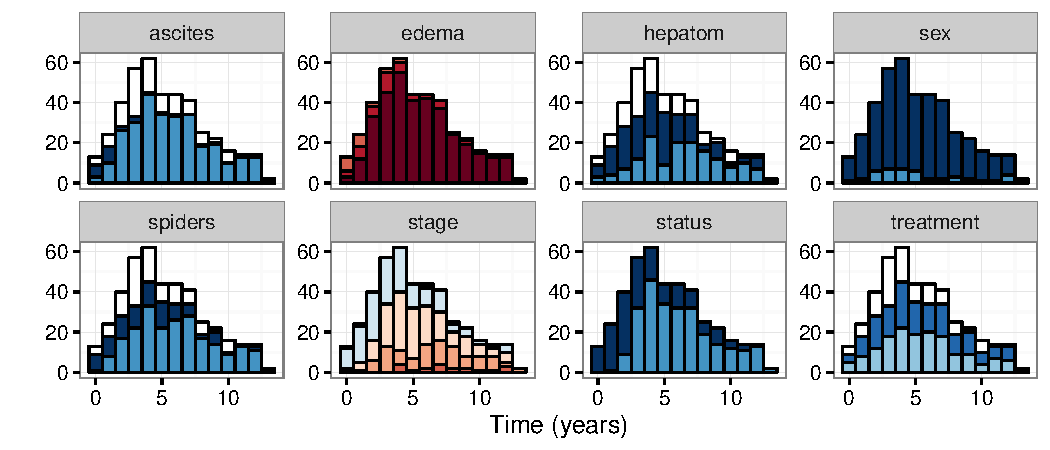
\includegraphics[width=\maxwidth]{fig-rfs/rfs-categoricalEDA-1} 

}

\caption[EDA plots for categorical variables (logicals and factors)]{EDA plots for categorical variables (logicals and factors). Bars indicate number of patients within 1 year of followup interval for each categorical variable. Colors correspond to class membership within each variable. Missing values are included in white.}\label{fig:categoricalEDA}
\end{figure}
\end{Schunk}

In categorical EDA plots (Figure~\ref{fig:categoricalEDA}), we are looking for patterns of missing data (white portion of bars). We often use surgical date for our X-axis variable to look for possible periods of low enrollment. There is not a comparable variable available in the \code{pbc} data set, so instead we used follow up time (\code{years}). Another reasonable choice may have been to use the patient \code{age} variable for the X-axis. The important quality of the selected variable is to spread the observations out to aid in finding data anomalies.

\begin{Schunk}
\begin{figure}[!htb]

{\centering 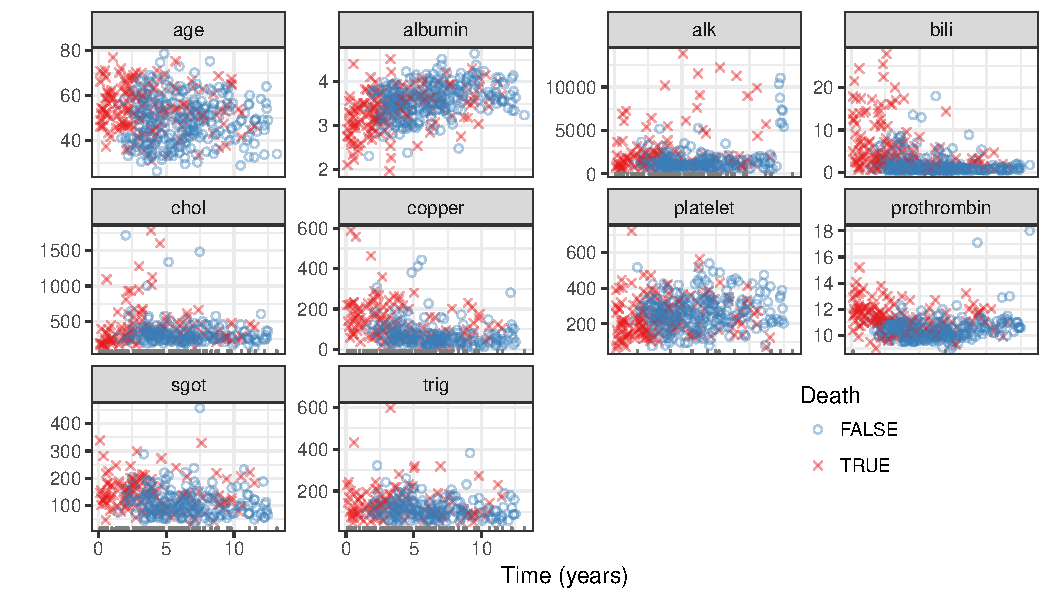
\includegraphics[width=\maxwidth]{fig-rfs/rfs-continuousEDA-1} 

}

\caption[EDA plots for continuous variables]{EDA plots for continuous variables. Symbols indicate observations with variable value on Y-axis against follow up time in years. Symbols are colored and shaped according to the death event  (\code{status} variable). Missing values are indicated by rug marks along the X-axis}\label{fig:continuousEDA}
\end{figure}
\end{Schunk}

In continuous data EDA plots (Figure~\ref{fig:continuousEDA}), we are looking for missingness (rug marks) and extreme or non-physical values. For survival settings, we color and shape the points as red `x's to indicate events, and blue circles to indicate censored observation.

Extreme value examples are evident in a few of the variables in Figure~\ref{fig:continuousEDA}. We are typically looking for values that are outside of the biological range. This is often caused by measurements recorded in differing units, which can sometimes be corrected algorithmically. Since we can not ask the original investigator to clarify these values in this particular study, we will continue without modifying the data.

\begin{table}

\caption{\label{T:missing}Missing value counts in \code{pbc} data set and pbc clinical trial observations (\code{pbc.trial}).}
\centering
\begin{tabular}[t]{lrr}
\toprule
  & pbc & pbc.trial\\
\midrule
treatment & 106 & 0\\
ascites & 106 & 0\\
hepatom & 106 & 0\\
spiders & 106 & 0\\
chol & 134 & 28\\
\addlinespace
copper & 108 & 2\\
alk & 106 & 0\\
sgot & 106 & 0\\
trig & 136 & 30\\
platelet & 11 & 4\\
\addlinespace
prothrombin & 2 & 0\\
stage & 6 & 0\\
\bottomrule
\end{tabular}
\end{table}



Both EDA figures indicate the \code{pbc} data set contains quite a bit of missing data. Table~\ref{T:missing} shows the number of missing values in each variable of the \code{pbc} data set. Of the 19 variables in the data, 12 have missing values. The \code{pbc} column details variables with missing data in the full \code{pbc} data set, though there are  patients that were not randomized into the trial. If we restrict the data to the trial only, most of the missing values are also removed, leaving only 4 variables with missing values. Therefore, we will focus on the 312 observations from the clinical trial for the remainder of this document. We will discuss how \pkg{randomForestSRC} handles missing values in Section~\ref{S:imputation}.

\subsection[PBC Model Summary]{\cite{fleming:1991} Model Summary (\code{gg\_survival})}

We conclude the data set investigation with a summary of~\cite{fleming:1991} model results from Chapter 4.4. We start by generating Kaplan--Meier (KM) survival estimates comparing the treatment groups of DPCA and placebo. We use the \pkg{ggRandomForests} \code{gg_survival} function to generate these estimates from the data set as follows.

\begin{Schunk}
\begin{Sinput}
R> # Create the trial and test data sets.
R> pbc.trial <- pbc %>% filter(!is.na(treatment))
R> pbc.test <- pbc %>% filter(is.na(treatment))
R> 
R> # Create the gg_survival object
R> gg_dta <- gg_survival(interval = "years",
+                       censor = "status",
+                       by = "treatment",
+                       data = pbc.trial,
+                       conf.int = 0.95)
\end{Sinput}
\end{Schunk}

% \begin{CodeInput}
% R> pbc.trial <- pbc %>% filter(!is.na(treatment))
% R> pbc.test <- pbc %>% filter(is.na(treatment))
% R>
% R> gg_dta <- gg_survival(interval = "years", censor = "status",
% +                        by = "treatment", data = pbc.trial,
% +                        conf.int = 0.95)
% \end{CodeInput}
The code block reduces the \code{pbc} data set to the \code{pbc.trial} which only include observations from the clinical trial. The remaining observations are stored in the \code{pbc.test} data set for later use. The \pkg{ggRandomForests} package is designed to use a two step process in figure generation. The first step is data generation, where we store a \code{gg_survival} data object in the \code{gg_dta} object. The \code{gg_survival} function uses the \code{data} set, follow up \code{interval}, \code{censor} indicator and an optional grouping argument (\code{by}). By default \code{gg_survival} also calculates $95\%$ confidence band, which we can control with the \code{conf.int} argument.

In the figure generation step, we use the \pkg{ggRandomForests} plot routine \code{plot.gg_survival} as shown in the following code block. The \code{plot.gg_survival} function uses the \code{gg_dta} data object to plot the survival estimate curves for each group and corresponding confidence interval ribbons. We have used additional \pkg{ggplot2} commands to modify the axis and legend labels (\code{labs}), the legend location (\code{theme}) and control the plot range of the y-axis (\code{coord_cartesian}) for this figure.

\begin{Schunk}
\begin{Sinput}
R> plot(gg_dta) +
+   labs(y = "Survival Probability", x = "Observation Time (years)",
+        color = "Treatment", fill = "Treatment") +
+   theme(legend.position = c(0.2, 0.2)) +
+   coord_cartesian(y = c(0, 1.01))
\end{Sinput}
\begin{figure}[!htb]

{\centering 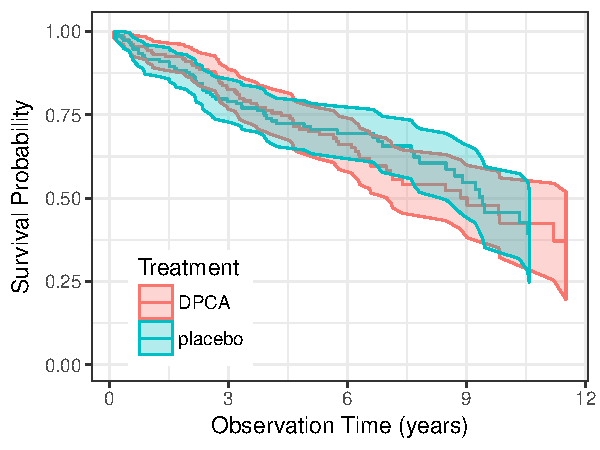
\includegraphics[width=\maxwidth]{fig-rfs/rfs-plot_gg_survival-1} 

}

\caption{Kaplan--Meier survival estimates comparing the \code{DPCA} treatment (red) with \code{placebo} (blue) groups for the \code{pbc.trail} data set. Median survival with shaded 95\% confidence band.}\label{fig:plot_gg_survival}
\end{figure}
\end{Schunk}
The \code{gg_survival} plot of Figure~\ref{fig:plot_gg_survival} is analogous to~\cite{fleming:1991} Figure 0.2.3 and Figure 4.4.1, showing there is little difference between the treatment and control groups.

The \code{gg_survival} function generates a variety of time-to-event estimates, including the cumulative hazard. The follow code block creates a cumulative hazard plot~\cite[Figure 0.2.1]{fleming:1991} in Figure~\ref{fig:plot_gg_cum_hazard} using the same data object generated by the original \code{gg_survival} function call. The red \code{DPCA} line is directly comparable to Figure 0.2.1, we've add the cumulative hazard estimates for the \code{placebo} population in blue.

\begin{Schunk}
\begin{Sinput}
R> plot(gg_dta, type = "cum_haz") +
+   labs(y = "Cumulative Hazard", x = "Observation Time (years)",
+        color = "Treatment", fill = "Treatment") +
+   theme(legend.position = c(0.2, 0.8)) +
+   coord_cartesian(ylim = c(-0.02, 1.22))
\end{Sinput}
\begin{figure}[!htb]

{\centering 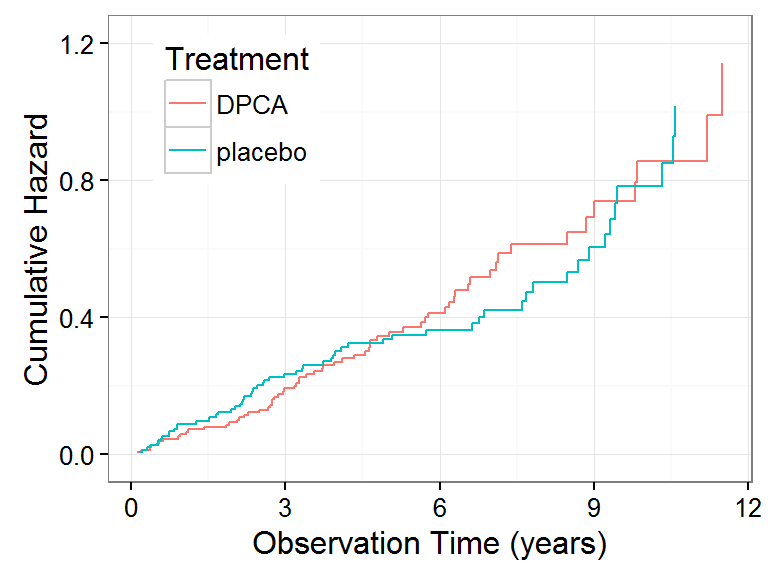
\includegraphics[width=\maxwidth]{fig-rfs/rfs-plot_gg_cum_hazard-1} 

}

\caption[Kaplan--Meier cumulative hazard estimates comparing the \code{DPCA} treatment (red) with \code{placebo} (blue) groups for the \code{pbc} data set]{Kaplan--Meier cumulative hazard estimates comparing the \code{DPCA} treatment (red) with \code{placebo} (blue) groups for the \code{pbc} data set.}\label{fig:plot_gg_cum_hazard}
\end{figure}
\end{Schunk}

In Figure~\ref{fig:plot_gg_survival}, we demonstrated grouping on the categorical variable (\code{treatment}). To demonstrate plotting grouped survival on a continuous variable, we examine KM estimates of survival within stratified groups of bilirubin measures. The groupings are obtained directly from~\cite{fleming:1991} Figure 4.4.2, where they presented univariate model results of predicting survival on a function of bilirubin.

We set up the \code{bili} groups on a temporary data set (\code{pbc.bili}) using the \code{cut} function with intervals matching the reference figure. For this example we combine the data generation and plot steps into a single line of code. The \code{error} argument of the \code{plot.gg_survival} function is used to control display of the confidence bands. We suppress the intervals for this figure with \code{error = "none"} and again modify the plot display with \pkg{ggplot2} commands to generate Figure~\ref{fig:gg_survival-bili}.

\begin{Schunk}
\begin{Sinput}
R> pbc.bili <- pbc.trial
R> pbc.bili$bili_grp <- cut(pbc.bili$bili, breaks = c(0, 0.8, 1.3, 3.4, 29))
R> 
R> plot(gg_survival(interval = "years", censor = "status", by = "bili_grp",
+                  data = pbc.bili), error = "none") +
+   labs(y = "Survival Probability", x = "Observation Time (years)",
+        color = "Bilirubin")
\end{Sinput}
\begin{figure}[!htb]

{\centering 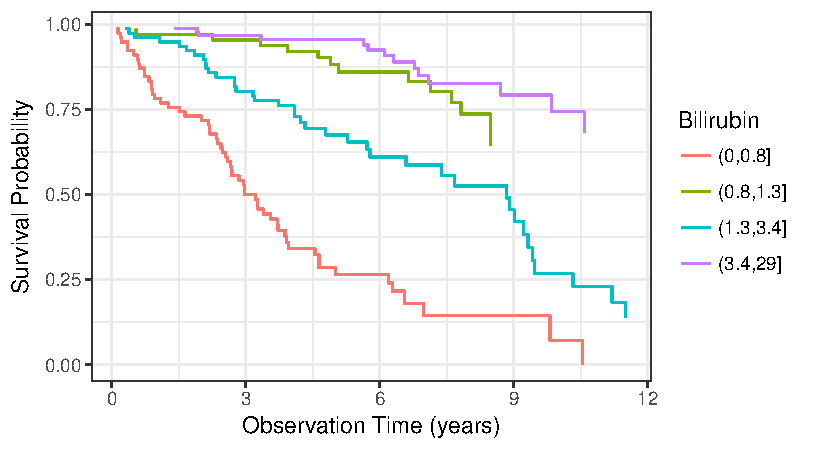
\includegraphics[width=\maxwidth]{fig-rfs/rfs-gg_survival-bili-1} 

}

\caption{Kaplan--Meier survival estimates comparing different groups of Bilirubin measures (\code{bili}) for the \code{pbc} data set. Groups defined in Chapter 4 of~\cite{fleming:1991}.}\label{fig:gg_survival-bili}
\end{figure}
\end{Schunk}

In Chapter 4,~\cite{fleming:1991} use partial likelihood methods to build a linear model with log transformations on some variables. We summarize the final, biologically reasonable model in Table~\ref{T:FHmodel} for later comparison with our random forest results.

\begin{table}

\caption{\label{T:FHmodel}\code{pbc} proportional hazards model summary of 312 randomized cases in \code{pbc.trial} data set. ~\citep[Table 4.4.3c]{fleming:1991} }
\centering
\begin{tabular}[t]{lrrr}
\toprule
  & Coef. & Std. Err. & Z stat.\\
\midrule
Age & 0.033 & 0.009 & 3.84\\
log(Albumin) & -3.055 & 0.724 & -4.22\\
log(Bilirubin) & 0.879 & 0.099 & 8.90\\
Edema & 0.785 & 0.299 & 2.62\\
log(Prothrombin Time) & 3.016 & 1.024 & 2.95\\
\bottomrule
\end{tabular}
\end{table}



\section{Random survival forest}\label{S:rfsrc}

A Random Forest~\citep{Breiman:2001} is grown by \emph{bagging}~\citep{Breiman:1996} a collection of \emph{classification and regression trees} (CART)~\citep{cart:1984}. The method uses a set of $B$ \emph{bootstrap}~\citep{bootstrap:1994} samples, growing an independent tree model on each sub-sample of the population. Each tree is grown by recursively partitioning the population based on optimization of a \emph{split rule} over the $p$-dimensional covariate space. At each split, a subset of $m \le p$ candidate variables are tested for the split rule optimization, dividing each node into two daughter nodes. Each daughter node is then split again until the process reaches the \emph{stopping criteria} of either \emph{node purity} or \emph{node member size}, which defines the set of \emph{terminal (unsplit) nodes} for the tree. In regression trees, node impurity is measured by mean squared error, whereas in classification problems, the Gini index is used~\citep{Friedman:2000} .

Random forest sorts each training set observation into one unique terminal node per tree. Tree estimates for each observation are constructed at each terminal node, among the terminal node members. The Random Forest estimate for each observation is then calculated by aggregating, averaging (regression) or votes (classification), the terminal node results across the collection of $B$ trees.

Random Survival Forests~\citep{Ishwaran:2007, Ishwaran:2008} (RSF) are an extension of Random Forest to analyze right censored, time to event data. A forest of survival trees is grown using a log-rank splitting rule to select the optimal candidate variables. Survival estimate for each observation are constructed with a Kaplan--Meier (KM) estimator within each terminal node, at each event time.

Random Survival Forests adaptively discover nonlinear effects and interactions and are fully nonparametric. Averaging over many trees enables RSF to approximate complex survival functions, including non-proportional hazards, while maintaining low prediction error. \cite{Ishwaran:2010a} showed that RSF is uniformly consistent and that survival forests have a uniform approximating property in finite-sample settings, a property not possessed by individual survival trees.

The \pkg{randomForestSRC} \code{rfsrc} function call grows the forest, determining the type of forest by the response supplied in the \code{formula} argument. In the following code block, we grow a random forest for survival, by passing a survival (\code{Surv}) object to the forest. The forest uses all remaining variables in the \code{pbc.trial} data set to generate the RSF survival model.

\begin{Schunk}
\begin{Sinput}
R> rfsrc_pbc <- rfsrc(Surv(years, status) ~ ., data = pbc.trial,
+                    nsplit = 10, na.action = "na.impute")
\end{Sinput}
\end{Schunk}












































































